\documentclass[times, utf8, zavrsni]{fer}
\usepackage{booktabs}
\usepackage{pgf,tikz}
\usetikzlibrary{arrows}
\usepackage{xcolor}
\usepackage{colortbl}
\usepackage{tabularx}

\usepackage{hyperref}
\hypersetup{
unicode=true, % za unicode podršku u bookmarkovima i sl., svakako postaviti na true
colorlinks=true, % za prikaz linkova u boji umjesto u pravokutnicima; slijede postavke po klasama linkova
linkcolor=black, % možete koristiti ime bilo koje definirane boje (pročitati post u kojem je predstavljen paket xcolor)
citecolor=black,
filecolor=black,
urlcolor=black,
linktocpage=false, % ako želite da oznaka stranice u tablici sadržaja bude link umjesto naslova, postavite na true
bookmarksopen=true, % pri otvaranju dokumenta će se prikazati toolbar s bookmarkovima, jako korisno
bookmarksopenlevel=1, % bookmarkovi su prikazani u stablastoj strukturi, a ovim određujete do koje će dubine stablo bookmarkova biti razgranato
bookmarksnumbered=true, % uz imena bookmarkova će se prikazati i njihov broj
pdftitle={SWIG - Poravnanje struktura korištenjem iterativne primjene Smith-Waterman algoritma},
pdfauthor={Bruno Rahle},
pdfsubject={tema},
pdfkeywords={kljucne rijeci - odvojite ih razmakom},
pdfstartpage={}, % ovisno koji stil numeriranja stranica koristite (\Roman, \roman, \arabic, \alph, \Alph), možete postaviti broj (oznaku) stranice koja će se prikazati prilikom otvaranja dokumenta; prazne vitičaste zagrade uvijek znače prvu stranicu, bez obzira na koji način bila numerirana
pdfstartview=FitH, % dokument će se prikazati tako da će mu širina odgovarati širini PDF preglednika
}
\def\subsectionautorefname{Odlomak}
\def\sectionautorefname{Potpoglavlje}
\def\chapterautorefname{Poglavlje}
\def\tableautorefname{Tablica}
\def\figureautorefname{Slika}

\begin{document}

\newcolumntype{R}{>{\centering\arraybackslash}X}%

\thesisnumber{2321}

\title{SWIG - Poravnanje struktura korištenjem iterativne primjene Smith-Waterman algoritma}

\author{Bruno Rahle}

\maketitle

% Ispis stranice s napomenom o umetanju izvornika rada. Uklonite naredbu \izvornik ako želite izbaciti tu stranicu.
\izvornik

% Dodavanje zahvale ili prazne stranice. Ako ne želite dodati zahvalu, naredbu ostavite radi prazne stranice.
\zahvala{}

\tableofcontents

\listoffigures

\listoftables

\chapter{Uvod}

Živimo u doba kada velikih promjena. Današnjim generacijama mladih nezamisliv
je život bez Interneta i društvenih mreža. Internet, a kamoli društvene mreže,
bili su nezamislivi njihovim roditeljima dok su bili mladi. Računala
su bila (većinom i ostala) neshvatljiva čuda djedovima i bakama, dok
je njihovim roditeljima čak i električna energija strana. 

Nije samo računarstvo doživjelo ogromne promjene. Tek pred nešto više od 
stotinu godinu izumljen je automobil. Danas gotovo da ne postoji obitelj
koja ne posjeduje barem jedan. 
%TODO daj jos jedan primjer

Još je veliki hrvatski pjesnik Petar Preradović u pjesmi "Mujezin" %TODO dodaj u bibliografiju, Vienac 1871.
zapisao "Stalna na tom svijetu samo mijena jest." Ono što danas smatramo
znanstvenom fantastikom za nekoliko bi godina moglo postati stvarnost. 
Kako se povećava ljudsko znanje, tako se povećava i broj pitanja na 
koje ljudi traže odgovore. Često problemi s kojima se znanost 
susreće prelaze granice isključivo jedne discipline. Zbog toga je postao
običaj da ljudi različitih profila sudjeluju na istom
istraživanju. 

%TODO dodaj jos nekoliko primjera gdje se razne grane znanosti susrecu

Postoji čitav niz problema iz biologije koji se danas više ili manje efikasno
rješavaju uz pomoć kompjutera. Ti problemi spadaju u područje koje nazivamo
bioinformatikom. Glavni problema koje rješava bioinformatika su:

\begin{itemize}
\item
Analiza nizova (engl. \textit{sequence analysis}). 

\item
Označavanje genoma (engl. \textit{genome annotation}).

\item
Računska evolucijska biologija (engl. \textit{computational
evolutionary biology}).

\item
Dubinska analiza teksta (engl. \textit{literature analysis}, 
\textit{data mining}).

\item
Analiza izražaja gena (engl. \textit{analysis of gene expression}).

\item
Analiza nadzora (engl. \textit{analysis of regulation}).

\item
Analiza izražaja proteina (engl. \textit{analysis of protein
expression}).

\item
Analiza mutacija u raku (engl. \textit{analysis of mutations in cancer}).

\item
Usporedna genomika (enl. \textit{comparative genomics}).

\item
Modeliranje bioloških sistema (engl. \textit{modeling biological
systems}).

\item
Visoko-propusna anliza slika (engl. \textit{high-throughput
image analysis}).

\item
Predviđanje struktura proteina (engl. \textit{protein structure prediction}).

\item 
Interakcija među molekulama (engl. \textit{molecular Interaction}).
\end{itemize}

Problem koji mi rješavamo, poravnavanje struktura, može se staviti u više 
područja koje smo naveli, budući da im se područja preklapaju. Taj problem
bitan je jer, ako ga uspješno riješimo, napravilo smo veliki posao jer
bi 




- pričaj još o: zašto je problem koji si rješavao bitan,
kome koristi, kako se može koristiti i potencijalno za što se
sve može koristiti.

- spomeni i grafičke kartice

- cca 2 stranice

- nešto sitno i o grafičkim karticama

\chapter{Poravanavanje sturktura}
U ovom radu bavit ćemo se rješavanjem slijedećeg problema: 

Zadana su nam dva proteina, tj. pozicije u prostoru svakog od atoma
koje protein sadrži. Zanimaju nas samo atomi ugljika, a ostali atomi
nam nisu interesantni. Želimo jednog od njih transforimarati 
koristeći samo translacije i rotacije tako da se što je moguće više
preklapa s drugim. Protein koji ćemo rotirati zvat ćemo protein $B$,
a protein $A$ bit će onaj s kojim ga želimo preklopiti. 

Kao rješenje želimo dobiti preklapanje koje će poravnati
neki podniz elemenata iz proteina $A$ i $B$ i koje će biti maksimalno
za ta dva proteina. Zbog toga nas zanima i rekonstrukcija rješenja. 

Da bismo dobili rješenje, koristit ćemo simulirano kaljenje 
zajedno sa Smith-Watermanovim algoritmom za proračun energije. 
Taj par algoritama trebao bi moći u "pristojnom" vremenu pronaći
neko poravnanje koje je relativno blisko optimalnom. 

Inovativnost ovog rada temelji se na tome da ćemo kao arhitekturu
koristi GPU, tj. grafičku procesnu jedinicu. Prednost GPU arhitekture
u odnosu na CPU jest to što je GPU masivno paralelan, što znači
da imamo velik broj dretvi (broje se u stotinama!) koje nam omogućavaju
da stvari rješavamo paralelno. Najzrelija tehnologija koja nudi
korištenje grafičkih kartica u svrhu procesiranja podataka je CUDA.
Unatoč nekim ograničenjima (npr. radi samo na Nvidijinim grafičkim
karticama), odlučili smo koristiti upravo nju za potrebe implementacije
rješenja ovog problema. 

- detaljan opis problema
- cca 1-2 stranice

\chapter{Smith-Watermanov algoritam}
Smith-Watermanov algoritam služi nam da bismo pronašli lokalno poravnanje. 
Osmislili su ga Temple F. Smith i Michael S. Waterman 1981. \cite{smithwaterman1981}.
Temelji se na Needleman-Wunschevom algoritmu (\cite{needlemanwunsch1970})
te i sam spada u kategoriju algoritama dinamičkog programiranja. Glavna razlika
između ta dva algoritma jest što Needleman-Wunschov algoritam prolazi globalno
poravananje.

- napisi jos teksta ovdje.

\section{Needleman-Wunschov algoritam}
\label{sec:nwalg}
Algoritam, kao što je već rečeno, traži globalno poravnanje. To znači da se svi 
članovi ulaznih nizova moraju poravnati. Dopuštene operacije kada tražimo poravnanje
su preklapanje s elementom iz suprotnog niza i ubacivanje praznina u neki od nizova.
Sve parove elemenata u dobivenom preklapanju bodujemo i na osnovu te ocjene
određujemo sličnost nizova. Konačan rezultat ovog algoritma jest poravnanje koje
maksimizira takvu ocjenu, tj. daje maksimalno globalno poravnanje.

Zanimljivost je da je to prvi algoritam dinamičkog programiranja ikada primjenjen
u bioinformatici.

\subsection{Ulazni podaci}
\label{subsec:nwinp}
\begin{enumerate}
	\item Dva niza ($A$ i $B$) proteina ili nukleotida. Zbog jednostavnosti, pretpostavit
		ćemo da su to nukleotidi iz DNK - adenin (A), timin (T), gvanin (G) i citozin (C).
		U primjeru ćemo koristiti $A = "ATGCCGTA"$ i $B = "TGCACTA"$. Dužinu niza $A$
		označit ćemo s $N$, a dužinu niza $B$ s $M$. 
	\item Supstitucijska matrica $S$, koja nam daje bodove koje dobijemo kada jedan
		nukletoid preklopimo s drugim. U našem će slučaju imati
		dimenzije $4 \times 4$, budući da ćemo razmatrati
		slučaj kada imamo samo četiri nukleotida. U principu će na dijagonali
		imati pozitivne brojeve, a na ostalim poljima negativne. To znači da nam
		se najviše isplati preklapati nukletide istog tipa, jer za to dobivamo bodove,
		a inače ih	gubimo. Primjer jedne takve matrice koju ćemo koristiti i u primjeru:

		\begin{table}
		\centering		
		\begin{tabular}{c|cccc}
		& A & C & G & T \\\specialrule{1pt}{0pt}{0pt}
		A & 10 & -3 & -9 & -1 \\
		C & -5 & 8 & -8 & -7 \\
		G & -5 & -4 & 7 & -5\\
		T & -4 & -11 & -8 & 9
		\end{tabular}
		\caption[Supstitucijska matrica]{Primjer supstitucijske matrice koju koristimo}
		\end{table}				

		
	\item Negativan broj $d$, koji označava bodove koje dobijemo (tj. izgubimo) kada nukleotid
		preklopimo s prazninom. U primjeru ćemo koristiti $d = -5$.
\end{enumerate}

\subsection{Izlazni podaci}
\label{subsec:nwout}
\begin{enumerate}
	\item Broj $H$, ocjena najboljeg globalnog poravnanja.
	\item Dva nova niza jednake dužine, $A'$ i $B'$, nastala ubacivanjem praznina
		(označenih najčešće sa '-') u nizove $A$ i $B$ koja predstavljaju najbolje pronađeno
		poravnanje.
\end{enumerate}

\subsection{Algoritam}
\label{subsec:nwalg}
Neka nam matrica $F$ služi za računanje poravnanja. 
Tada će nam $F_{i,j}$ označavati maksimalan broj bodova koje možemo dobiti kada
poravnamo prvih $i$ članova niza $A$ i prvih $j$ članova niza $B$. $F_{i,j}$ možemo
računati rekurzijom na slijedeći način:
$$
F_{i,j} = \left\{
	\begin{array}{lr}
		0 & \mbox{ako je } i=0 \mbox{ i } j=0 \\
		F_{i-1,j} + d & \mbox{ako je } i>0 \mbox{ i } j=0 \\
		F_{i,j-1} + d & \mbox{ako je } i=0 \mbox{ i } j>0 \\
		max \left(
			\begin{array}{l}
				F_{i-1,j-1} + S_{A_{i-1}, B_{j-1}} \\
				F_{i-1, j} + d \\
				F_{i, j-1} + d
			\end{array}
		\right) & \mbox{ako je } i>0 \mbox{ i } j>0
	\end{array}
\right.
$$

U $F_{N,M}$ će nam stoga pisati maksimalno globalno poravnanje. Primjetite da
u niti jednom slučaju nećemo poravnati dvije praznine. Ako bismo to učinili, 
samo bismo izgubili bodove, budući da je $d$ nužno negativan broj.

Da bismo znali rekonstruirati rješenje, koristit ćemo matricu $R$. U
polju $R_{i,j}$  pisat će koje smo polje matrice $F$ koristili da bi došli u
polje $F_{i,j}$. Kako su jedine mogućnosti $F_{i-1,j}$, $F_{i,j-1}$, $F_{i-1,j-1}$
i da nismo došli iz nikojeg polja (to vrijedi jedino za polje $F_{0,0}$), koristit
ćemo redom oznake $A$, $B$, $O$ i $X$. 

$$
R_{i,j} = \left\{
	\begin{array}{ll}
		X & \mbox{ako je} \left( \begin{array}{l} i=0 \\ j=0 \end{array} \right) \\
		O & \mbox{ako je} \left( \begin{array}{l} i>0 \\ j>0 \\
				F_{i-1,j-1} + S_{A_{i-1}, B_{j-1}} \geq F_{i-1,j} + d \\
				F_{i-1,j-1} + S_{A_{i-1}, B_{j-1}} \geq F_{i,j-1} + d \\
			\end{array} \right) \\
		A & \mbox{ako je} \left( \begin{array}{l} i>0 \\ j=0 \end{array} \right)
			\mbox{ili} \left( \begin{array}{l} i>0 \\ j>0 \\
				F_{i-1,j} + d > F_{i-1,j-1} + S_{A_{i-1}, B_{j-1}} \\
				F_{i-1,j} + d \geq F_{i,j-1} + d
			\end{array} \right) \\
		B & \mbox{ako je} \left( \begin{array}{l} i=0 \\ j>0 \end{array} \right)
			\mbox{ili} \left( \begin{array}{l} i>0 \\ j>0 \\
				F_{i,j-1} + d > F_{i-1,j-1} + S_{A_{i-1}, B_{j-1}} \\
				F_{i,j-1} + d > F_{i-1,j} + d
			\end{array} \right) \\
	\end{array}
\right.
$$

Rekonstrukciju provodimo tako krenemo iz polja $R_{N,M}$ i krećemo se
po matrici unazad dok ne dođemo do polja na kojem piđe $X$, tj. $R_{0,0}$.
Ako na polju pročitamo $O$,
pomičemo se po dijagonili, tj. u izlazni niz spremimo par $(A_{i-1}, B_{j-1})$ te
smanjimo i $i$ i $j$. Ako pročitamo $A$, spremamo par $(A_{i-1}, -)$ te smanjimo
samo $i$ za jedan. U slučaju da pročitamo $B$, spremamo par $(-, B_{j-1})$ te
smanjujemo $j$ za jedan. Ako smo pročitali $X$, došli smo do kraja i generirali
smo izlazni niz, ali u obrnutom redosljedu. 

\subsection{Primjer}
\autoref{table:Fnw} i \autoref{table:Rnw} sadrže potpuno izračunate matrice $F$ i $R$.
Iz tih podataka lagano je napraviti
potpunu rekonstrukciju (polja označena sivom bojom). Stoga zaključujemo da je
traženo globlano poravnanje
$A' = \mbox{"ATGCCGTA"}$ i $B' = \mbox{"-TGCACTA"}$.


\begin{table}
\centering
\begin{tabular}{c|cccccccc}
 & - & T & G & C & A & C & T & A \\\specialrule{0.5pt}{0pt}{0pt}
- & \cellcolor{lightgray} 0 & -5 & -10 & -15 & -20 & -25 & -30 & -35 \\ 
A & \cellcolor{lightgray} -5 & -1 & -6 & -11 & -5 & -10 & -15 & -20 \\ 
T & -10 & \cellcolor{lightgray} 4 & -1 & -6 & -10 & -15 & -1 & -6 \\ 
G & -15 & -1 & \cellcolor{lightgray} 11 & 6 & 1 & -4 & -6 & -6 \\ 
C & -20 & -6 & 6 & \cellcolor{lightgray} 19 & \cellcolor{lightgray} 14 & 9 & 4 & -1 \\ 
C & -25 & -11 & 1 & 14 & 14 & \cellcolor{lightgray} 22 & 17 & 12 \\ 
G & -30 & -16 & -4 & 9 & 9 & \cellcolor{lightgray} 17 & 17 & 12 \\ 
T & -35 & -21 & -9 & 4 & 5 & 12 & \cellcolor{lightgray} 26 & 21 \\ 
A & -40 & -26 & -14 & -1 & 14 & 9 & 21 & \cellcolor{lightgray} 36 \\ 
\end{tabular}
\caption[Matrica $F$ za Needleman-Wunschov algoritam]{Potpuno izračunata matrica $F$ za Needleman-Wunschov algoritam}
\label{table:Fnw}
\end{table}


\begin{table}
\centering
\begin{tabular}{c|cccccccc}
 & - & T & G & C & A & C & T & A \\\specialrule{0.5pt}{0pt}{0pt}
- & \cellcolor{lightgray} X & B & B & B & B & B & B & B \\ 
A & \cellcolor{lightgray} A & O & B & B & O & B & B & O \\ 
T & A & \cellcolor{lightgray} O & B & B & A & A & O & B \\ 
G & A & A & \cellcolor{lightgray} O & B & B & B & A & O \\ 
C & A & A & A & \cellcolor{lightgray} O & \cellcolor{lightgray} B & O & B & B \\ 
C & A & A & A & O & O & \cellcolor{lightgray} O & B & B \\ 
G & A & A & O & A & O & \cellcolor{lightgray} A & O & O \\ 
T & A & O & A & A & O & A & \cellcolor{lightgray} O & B \\ 
A & A & A & A & A & O & B & A & \cellcolor{lightgray} O \\ 
\end{tabular}
\caption[Matrica $R$ za Needleman-Wunschov algoritam]{Potpuno izračunata matrica $R$ za
Needleman-Wunschov algoritam}
\label{table:Rnw}
\end{table}

\subsection{Analiza složenosti}
Trivijalno je vidljivo da su memorijska i vremenska složenost opisanog algoritma 
jednake $O(NM)$. 



\section{Smith-Watermanov algoritam}
\label{sec:swalg}
Razlika njega i prethodno opisanog Needleman-Wunschevog algoritma jest u tome
što ovaj algoritam traži najbolje lokalno poravnanje. To znači da ne koristi
nužno cijele nizove proteina ili nukleotida već samo najsličnije uzastopne
podnizove. U praksi se koriste nešto poboljšane verzije ovog algoritma.

\subsection{Ulazni podaci}
Vidi \autoref{subsec:nwinp}.

\subsection{Izlazni podaci}
Vidi \autoref{subsec:nwout}.

\subsection{Algoritam}
\label{subsec:swalg}
U ovom ćemo algoritmu koristiti matricu $H$ za računanje poravnanja.
Za razliku od Needleman-Wunschevog algoritma, $H_{i,j}$ ovaj će put
označavati rezultat
najboljeg lokalnog poravnanja koje koristi $A_{i-1}$ i $B_{j-1}$.
Matricu ćemo popuniti na slijedeći način:

$$
H_{i,j} =
\left\{ \begin{array}{ll}
	0 & \mbox{ako je } i=0 \mbox{ ili } j=0 \\
	\max \left( \begin{array}{l}
		0 \\
		H_{i-1,j-1} + S_{A_{i-1}, B_{j-1}} \\
		H_{i-1, j} + d \\
		H_{i, j-1} + d
	\end{array} \right) & \mbox{ako je } i>0 \mbox{ i } j>0
\end{array} \right.
$$

Primjetite bitnu razliku u odnosu na Needleman-Wunschev algoritam - u ovom
slučaju matrica $H$ neće sadržavati negativne brojeve. Rješenje, tj. najbolje
lokalno poravnanje više neće pisati na polju $H_{N, M}$. Ono će biti na polju 
$(t, u)$ na kojem se nalazi najveći broj u matrici.

Da bismo znali rekonstruirati takvo lokalno poravnanje, koristit ćemo matricu
$R$ koju gradimo na sličan način kao i kod prethodnog algoritma:

$$
R_{i,j} =  \left\{
	\begin{array}{ll}
		X & \mbox{ako je} H_{i,j}=0 \\
		O & \mbox{ako je} \left( \begin{array}{l} i>0 \\ j>0 \\
				H_{i-1,j-1} + S_{A_{i-1}, B_{j-1}} \geq H_{i-1,j} + d \\
				H_{i-1,j-1} + S_{A_{i-1}, B_{j-1}} \geq H_{i,j-1} + d \\
			\end{array} \right) \\
		A & \mbox{ako je} \left( \begin{array}{l} i>0 \\ j=0 \end{array} \right)
			\mbox{ili} \left( \begin{array}{l} i>0 \\ j>0 \\
				H_{i-1,j} + d > H_{i-1,j-1} + S_{A_{i-1}, B_{j-1}} \\
				H_{i-1,j} + d \geq H_{i,j-1} + d
			\end{array} \right) \\
		B & \mbox{ako je} \left( \begin{array}{l} i=0 \\ j>0 \end{array} \right)
			\mbox{ili} \left( \begin{array}{l} i>0 \\ j>0 \\
				H_{i,j-1} + d > H_{i-1,j-1} + S_{A_{i-1}, B_{j-1}} \\
				H_{i,j-1} + d > H_{i-1,j} + d
			\end{array} \right) \\
	\end{array}
\right.
$$

Rekonstrukcija se, slično kao i kod Needleman-Wunschevog algoritma,
izvodi tako da krenemo iz polja $(t, u)$ i krećemo se  po matrici $R$ dok
ne dođemo do polja na kojem piše $X$ koje ovaj put ne mora nužno biti 
polje $R_{0,0}$. Dobiveni niz okrenemo i dobit ćemo traženo poravnanje.

\subsection{Primjer}
\autoref{table:Hsw} i \autoref{table:Rsw} prikazuju potpuno izračunate
matrice $H$ i $R$ nakon izvršavanja Smith-Watermanovog algoritma. 
Iz njih je lako očitati traženo poravnanje: $A' = \mbox{"TGC-CGTA"}$ i
$B' = \mbox{"TGCAC-TA"}$.


\begin{table}
\centering
\begin{tabular}{c|cccccccc}
 & - & T & G & C & A & C & T & A \\\specialrule{1pt}{0pt}{0pt}
- & 0 & 0 & 0 & 0 & 0 & 0 & 0 & 0 \\ 
A & \cellcolor{lightgray} 0 & 0 & 0 & 0 & 10 & 5 & 0 & 10 \\ 
T & 0 & \cellcolor{lightgray} 9 & 4 & 0 & 5 & 0 & 14 & 9 \\ 
G & 0 & 4 & \cellcolor{lightgray} 16 & 11 & 6 & 1 & 9 & 9 \\ 
C & 0 & 0 & 11 & \cellcolor{lightgray} 24 & \cellcolor{lightgray} 19 & 14 & 9 & 4 \\ 
C & 0 & 0 & 6 & 19 & 19 & \cellcolor{lightgray} 27 & 22 & 17 \\ 
G & 0 & 0 & 7 & 14 & 14 & \cellcolor{lightgray} 22 & 22 & 17 \\ 
T & 0 & 9 & 4 & 9 & 10 & 17 & \cellcolor{lightgray} 31 & 26 \\ 
A & 0 & 4 & 0 & 4 & 19 & 14 & 26 & \cellcolor{gray} 41 \\ 
\end{tabular}
\caption[Matrica $H$ za Smith-Watermanov algoritam]{Potpuno izračunata matrica $H$ za Smith-Watermanov algoritam}
\label{table:Hsw}
\end{table}

\begin{table}
\centering
\begin{tabular}{c|cccccccc}
 & - & T & G & C & A & C & T & A \\\specialrule{1pt}{0pt}{0pt}
- & X & X & X & X & X & X & X & X \\ 
A & \cellcolor{lightgray} X & X & X & X & O & B & B & O \\ 
T & X & \cellcolor{lightgray} O & B & X & A & A & O & B \\ 
G & X & A & \cellcolor{lightgray} O & B & B & O & A & O \\ 
C & X & X & A & \cellcolor{lightgray} O & \cellcolor{lightgray} B & O & B & O \\ 
C & X & X & A & O & O & \cellcolor{lightgray} O & B & B \\ 
G & X & X & O & A & O & \cellcolor{lightgray} A & O & O \\ 
T & X & O & B & A & O & A & \cellcolor{lightgray} O & B \\ 
A & X & A & O & A & O & B & A & \cellcolor{lightgray} O \\ 
\end{tabular}
\caption[Matrica $R$ za Smith-Watermanov algoritam]{Potpuno izračunata matrica $R$ za Smith-Watermanov algoritam}
\label{table:Rsw}
\end{table}

\subsection{Analiza složenosti}
Trivijalno je vidljivo da su memorijska i vremenska složenost i ovog algoritma 
jednake $O(NM)$. 


\section{Procjepi}
Do sada smo razmatrali samo slučaj kada je cijena otvaranja procjepa i
njegova proširivanja jednaka ($d$). Taj slučaj nazivamo
\textit{linearnom ocjenom procjepa},
budući da, ako je $k$ dužina procjepa, $dk$ je cijena za taj procjep. 
U praksi se primjenjuju još dva načina ocjenjivana procjepa.

Jedan je da za svaki procjep, bez obzira na njegovu dužinu, platimo fiksnu
cijenu ($c$), a nazivamo ga \textit{konstantnom ocjenom procjepa}. 

Drugi je kombinacija prethodna dva načina: za svaki procjep plaćamo fiksnu
cijenu ($c$), ali za njegovo produženje plaćamo neku drugu cijenu ($d$).
Takvu funkciju ocjene procjepa nazivamo \textit{Afinom ocjenom procjepa}.
Prema tome, za procjep dužine $k$, platit ćem cijenu jednaku $c + (k-1)d$.
Kako je empirijski pokazano da je ta funkcija u biti parobala, ovakva je
ocjena ujedno i najpreciznija. Nažalost, ona otežava računanje matrice
$H$ (i $R$). Problem je najlakše riješiti tako da uvedemo dvije nove
matrice $H^A$ i $H^B$ koje će nam pomoći u računanju cijene procjepa.
Matrice ćemo onda računati na slijedeći način:

$$
H_{i,j} =
\left\{ \begin{array}{ll}
	0 & \mbox{ako je } i=0 \mbox{ ili } j=0 \\
	\max \left( \begin{array}{l}
		0 \\
		H_{i-1,j-1} + S_{A_{i-1}, B_{j-1}} \\
		H^A_{i-1, j} + c \\
		H^B_{i, j-1} + c
	\end{array} \right) & \mbox{ako je } i>0 \mbox{ i } j>0
\end{array} \right.
$$

$$
H^{A}_{i,j} =
\left\{ \begin{array}{ll}
	0 & \mbox{ako je } i=0 \mbox{ ili } j=0 \\
	\max \left( \begin{array}{l}
		0 \\
		H_{i-1,j-1} + S_{A_{i-1}, B_{j-1}} \\
		H^A_{i-1, j} + d \\
		H^B_{i, j-1} + c
	\end{array} \right) & \mbox{ako je } i>0 \mbox{ i } j>0
\end{array} \right.
$$

$$
H^{B}_{i,j} =
\left\{ \begin{array}{ll}
	0 & \mbox{ako je } i=0 \mbox{ ili } j=0 \\
	\max \left( \begin{array}{l}
		0 \\
		H_{i-1,j-1} + S_{A_{i-1}, B_{j-1}} \\
		H^A_{i-1, j} + c \\
		H^B_{i, j-1} + d
	\end{array} \right) & \mbox{ako je } i>0 \mbox{ i } j>0
\end{array} \right.
$$

Rekonstrukcijska matrica vrlo je slična onoj u izvorno opisanom
algoritmu, a kako ćemo u udućem potpoglavlju maknuti potrebu za njom,
nećemo je posebno navoditi. 

\section{Memorijska optimizacija}
S obzirom da nizovi nukleotida mogu sadržavati i do nekoliko milijuna
elemenata, matrica dimenzija $N M$ fizički ne stane u memoriju. 
Međutim, čim primjetimo da za potrebe generiranja matrice $H$ (a ujedno i
$H^A$ odnosno $H^B$) koristimo
samo polja iz trenutnog i prethodnog retka, postaje jasno da nam ostali 
reci koje smo obradili ranije njih nisu potrebni. Stoga možemo pamtiti 
samo ta dva retka i time korištenu memoriju za proračun
matrice $H$ smanjimo na samo $O(\min(N, M))$. Ipak, problem se javlja
kada trebamo rekonstruirati rješenje pomoću matrice $R$, budući da
se prilikom rekonstrukcije potencijalno vraćamo se kroz sva njena polja. U
nastavku ćemo opisati rješenje tog problema.

\begin{table}
\centering
\begin{tabularx}{400pt}{|R|R|R|R|R|R|R|R|R|R|R|R|R|R|R|R|R|R|R|R|}
 \hline
  &  &  &  &  &  &  &  &  &  &  &  &  &  &  &  &  &  &  &  \\ \hline
  &  &  &  &  &  &  &  &  &  &  &  &  &  &  &  &  &  &  &  \\ \hline
  &  &  &  &  &  &  &  &  &  &  &  &  &  &  &  &  &  &  &  \\ \hline
  &  &  &  &  &  &  &  & \cellcolor[rgb]{0.784314,0.784314,0.784314}  & \cellcolor[rgb]{0.784314,0.784314,0.784314}  & \cellcolor[rgb]{0.784314,0.784314,0.784314}  & \cellcolor[rgb]{0.784314,0.784314,0.784314}  & \cellcolor[rgb]{0.784314,0.784314,0.784314}  & \cellcolor[rgb]{0.784314,0.784314,0.784314}  & \cellcolor[rgb]{0.784314,0.784314,0.784314}  & \cellcolor[rgb]{0.784314,0.784314,0.784314}  & \cellcolor[rgb]{0.784314,0.784314,0.784314}  & \cellcolor[rgb]{0.784314,0.784314,0.784314}  & \cellcolor[rgb]{0.784314,0.784314,0.784314}  & \cellcolor[rgb]{0.784314,0.784314,0.784314}  \\ \hline
 \cellcolor[rgb]{0.784314,0.784314,0.784314}  & \cellcolor[rgb]{0.784314,0.784314,0.784314}  & \cellcolor[rgb]{0.784314,0.784314,0.784314}  & \cellcolor[rgb]{0.784314,0.784314,0.784314}  & \cellcolor[rgb]{0.784314,0.784314,0.784314}  & \cellcolor[rgb]{0.784314,0.784314,0.784314}  & \cellcolor[rgb]{0.784314,0.784314,0.784314}  & \cellcolor[rgb]{0.784314,0.784314,0.784314}  & \cellcolor[rgb]{0.784314,0.784314,0.784314}  & \cellcolor[rgb]{0.392157,0.392157,0.392157}  &  &  &  &  &  &  &  &  &  &  \\ \hline
  &  &  &  &  &  &  &  &  &  &  &  &  &  &  &  &  &  &  &  \\ \hline
\end{tabularx}
\caption[Memorijska optimizacija]{Pod pretpostavkom da polja računamo iterativno 
po recima, matrica prikazuje koja polja moramo čuvati u
memoriji (svjetlo-siva boja) da bismo mogli izračunati preostala.
Polje koje trenutno računamo
pobojano je tamno-sivom bojom. U praksi ćemo, zbog jednostavnosti,
čuvati cijeli prošli redak.}
\label{table:memopt}
\end{table}

\subsection{Hirschbergov algoritam}
Dan Hirschberg osmislio je algoritam koji rješava problem rekonstrukcije
globalnog poravnanja u $O(NM)$ vremena koristeći $O(\min(N, M))$ memorije.
Njegova ideja temeljena je na metodi \textit{podijeli-pa-vladaj}.

No, prije nego je objasnimo, promotrimo što će se dogoditi s globalnim
poravnanjem ako okrenemo nizove $A$ i $B$. Okrenute nizove nazivat ćemo
$A^R$ i $B^R$, a matrice $F^R$ i $R^R$. Očito je da se ocjena poravnanja
neće  promijeniti, a prilikom rekonstrukcije dobit ćemo obrnuti niz. Uz sitne
modifikacije, možemo izračunati matricu $F^R$ bez da fizički okrećemo
nizove. 

Hirschbergov algoritam radi na slijedeći način:
\begin{enumerate}
\item
Bez smanjenja općenitosti, možemo pretpostaviti da je niz $A$ duži od
niza $B$. Neka nam $p$ označava polovicu dužine niza $A$, zaokruženu na dolje.
Podijelimo niz $A$ na dvije polovice, dužine $p$.

\item
Na obje polovice niza ($A_{0..p}$ i $A_{p..N}^{R}$) pokrenemo gore
opisani algoritam za pronalaženje
lokalnog poravnanja koje koristi $O(\min(N,M))$ memorije, ali bez
rekonstrukcije. Nad drugom polovicom niza radimo algoritam za obrnuto
nizove, tako da je za obje polovice posljednji izračunati red onaj odabran u
prethodnom koraku. 

\begin{table}
\centering
\begin{tabularx}{160pt}{|R|R|R|R|R|R|R|R|}
 \hline
  & $\Rightarrow$ &  &  &  &  &  &  \\ \hline
 $\Downarrow$ &  &  &  &  &  &  &  \\ \hline
  &  &  &  &  &  &  &  \\ \hline
  &  &  &  &  &  &  &  \\ \hline
 \cellcolor[rgb]{0.627451,0.627451,0.627451}  & \cellcolor[rgb]{0.627451,0.627451,0.627451}  & \cellcolor[rgb]{0.627451,0.627451,0.627451}  & \cellcolor[rgb]{0.627451,0.627451,0.627451}  & \cellcolor[rgb]{0.627451,0.627451,0.627451}  & \cellcolor[rgb]{0.627451,0.627451,0.627451}  & \cellcolor[rgb]{0.627451,0.627451,0.627451}  & \cellcolor[rgb]{0.627451,0.627451,0.627451}  \\ \hline
  &  &  &  &  &  &  &  \\ \hline
  &  &  &  &  &  &  &  \\ \hline
  &  &  &  &  &  &  & $\Uparrow$ \\ \hline
  &  &  &  &  &  & $\Leftarrow$ &  \\ \hline
\end{tabularx}
\caption[TODO: smisli dobar naslov]{Računanje Smith-Watermannovog algoritma
na dvije polovice niza ($A_{0..p}$ i $A_{p..N}^{R}$). Svijetlo siva
linija predstavlja red $p$, prvi odnosno posljednji red za koji
računamo lokalno poravnanje. }
\label{table:Halg:1}
\end{table}

\item
Definirajmo funkciju $\phi(j)$ kao sumu lokalnih poravnanja obje matrice u redu
$p$, tj. kao:
$$ \phi(j) = F_{p,j} + F^{R}_{p,j} $$
Barem će jedan član globalnog poravnanja, biti u retku $p$, a Hirschberg
je pokazao da će to biti onaj u stupcu $j$ za kojeg je $\phi(j)$ najveći.
Time smo pronašli jedan član koji je sigurno u globalnom poravnanju. 

\begin{table}
\centering
\begin{tabularx}{160pt}{|R|R|R|R|R|R|R|R|}
 \hline
  &  &  &  &  &  &  &  \\ \hline
  &  &  &  &  &  &  &  \\ \hline
  &  &  &  &  &  &  &  \\ \hline
  &  &  &  &  &  &  &  \\ \hline
 \cellcolor[rgb]{0.627451,0.627451,0.627451}  & \cellcolor[rgb]{0.627451,0.627451,0.627451}  & \cellcolor[rgb]{0.627451,0.627451,0.627451}  & \cellcolor[rgb]{0.627451,0.627451,0.627451}  & \cellcolor[rgb]{0.627451,0.627451,0.627451}  & \cellcolor[rgb]{0.313725,0.313725,0.313725}  & \cellcolor[rgb]{0.627451,0.627451,0.627451}  & \cellcolor[rgb]{0.627451,0.627451,0.627451}  \\ \hline
  &  &  &  &  &  &  &  \\ \hline
  &  &  &  &  &  &  &  \\ \hline
  &  &  &  &  &  &  &  \\ \hline
  &  &  &  &  &  &  &  \\ \hline
\end{tabularx}
\caption[TODO: smisli dobar naslov 2]{Nakon što smo završili s računanjem
poravnanja na oba dijela niza, trebamo pronaći polje u kojem je $\phi(j)$
maksimalno. To polje označeno je tamno-sivom bojom.}
\label{table:Halg:2}
\end{table}

\item
S obzirom na svojstva globalnog poravnanja, intuitivno je jasno da
polja koja se nalaze gore-desno i dolje-lijevo od pronađenog polja 
sigurno nisu u točnom globalnom poravnanju, stoga ta polja
možemo izbaciti iz daljnjeg razmatranja. Ako rekurzivno primjenimo
algoritam na parove podnizova $A_{0..p}$ i $B_{0,j}$ te $A_{p..N}$ i
$B_{j..M}$, možemo ponavljajući postupak napraviti rekonstrukciju
cijelog niza.

\begin{table}
\centering
\begin{tabularx}{160pt}{|R|R|R|R|R|R|R|R|}
 \hline
  &  &  &  &  &  & \cellcolor[rgb]{0.862745,0.862745,0.862745}  & \cellcolor[rgb]{0.862745,0.862745,0.862745}  \\ \hline
  &  &  &  &  &  & \cellcolor[rgb]{0.862745,0.862745,0.862745}  & \cellcolor[rgb]{0.862745,0.862745,0.862745}  \\ \hline
  &  &  &  &  &  & \cellcolor[rgb]{0.862745,0.862745,0.862745}  & \cellcolor[rgb]{0.862745,0.862745,0.862745}  \\ \hline
  &  &  &  &  &  & \cellcolor[rgb]{0.862745,0.862745,0.862745}  & \cellcolor[rgb]{0.862745,0.862745,0.862745}  \\ \hline
  &  &  &  &  & \cellcolor[rgb]{0.313725,0.313725,0.313725}  &  &  \\ \hline
 \cellcolor[rgb]{0.862745,0.862745,0.862745}  & \cellcolor[rgb]{0.862745,0.862745,0.862745}  & \cellcolor[rgb]{0.862745,0.862745,0.862745}  & \cellcolor[rgb]{0.862745,0.862745,0.862745}  & \cellcolor[rgb]{0.862745,0.862745,0.862745}  &  &  &  \\ \hline
 \cellcolor[rgb]{0.862745,0.862745,0.862745}  & \cellcolor[rgb]{0.862745,0.862745,0.862745}  & \cellcolor[rgb]{0.862745,0.862745,0.862745}  & \cellcolor[rgb]{0.862745,0.862745,0.862745}  & \cellcolor[rgb]{0.862745,0.862745,0.862745}  &  &  &  \\ \hline
 \cellcolor[rgb]{0.862745,0.862745,0.862745}  & \cellcolor[rgb]{0.862745,0.862745,0.862745}  & \cellcolor[rgb]{0.862745,0.862745,0.862745}  & \cellcolor[rgb]{0.862745,0.862745,0.862745}  & \cellcolor[rgb]{0.862745,0.862745,0.862745}  &  &  &  \\ \hline
 \cellcolor[rgb]{0.862745,0.862745,0.862745}  & \cellcolor[rgb]{0.862745,0.862745,0.862745}  & \cellcolor[rgb]{0.862745,0.862745,0.862745}  & \cellcolor[rgb]{0.862745,0.862745,0.862745}  & \cellcolor[rgb]{0.862745,0.862745,0.862745}  &  &  &  \\ \hline
\end{tabularx}
\caption[Odbacivanje polja u Hirschbergovom algoritmu]{Budući da
smo sigurni da polja gore-desno i dolje-lijevo nisu u 
traženom globalnom poravnanju, njih ne trebamo dalje promatrati.
Na slici su označena svijetlo sivom bojom.}
\label{table:Halg:3}
\end{table}


\end{enumerate}

Ono što možda nije jasno jest vremenska složenost gore opisanog algoritma.
Pokazuje se da pri odbacivanju polja odbacimo u pravlu polovicu trenutno
razmatranih polja. Prema tome, broj operacija koje napravimo možemo napisati
u obliku geometrijskog niza:
$$ NM + NM/2 + NM/4 + ... < 2 NM \in O(NM) $$
Time dolazimo do zaključka da je složenost i dalje ostala jednaka do
razlike u konstantni, ali je znanto smanjena količina iskorištene
memorije, stoga se ova ušteda isplatiti koristiti.




\section{Substitucija substitucijske matrice}
- TODO: neko bolje ime za ovo potpoglavlje

U ovom ćemo radu umjesto supstitucijske matrice za usporedbu dva elementa
koristiti fizičku udaljenost između dva atoma. Stoga će nizovi A i B biti
zapravo nizovi koordinata iz kojih ćemo moći za svaki par elemenata
izračunati koordinate. 

Neka nam $d$ označava udaljenost između dva atoma, a $d_0$ neka nam
je konstanta (recimo $d_0 = 10$). Tada ćemo im udaljenost ocijeniti s
$30-e^{d/d_0}$. 


\chapter{Algoritam simuliranog kaljenja}
Algoritam simuliranog kaljenja generička je metoda bazirana na vjerojatnosti koja
traži ekstrem neke funkcije u velikom prostoru traženja. Zbog toga što nam ne
garantira da će pronaći najbolje rješenje, obično se koristi kada nam je
želimo dobiti rješenje koje je prihvatljivo u relativno kratkom
vremenu.

Inspiracija za algoritam dolazi iz metalurgije. Metali se prvo grubo obrađuju
na visokoj temperaturi, a, kako se hlade, tako obrada postaje sve finija
i  finija. Drugim riječima, \textit{željezo se kuje dok je vruće}. 
Taj proces pokušavamo simulirati u ovom algoritmu.

%preuzeto s http://www.flickr.com/photos/beginasyouare/6121659469/sizes/l/in/photostream/
\begin{figure}[h]
\centering
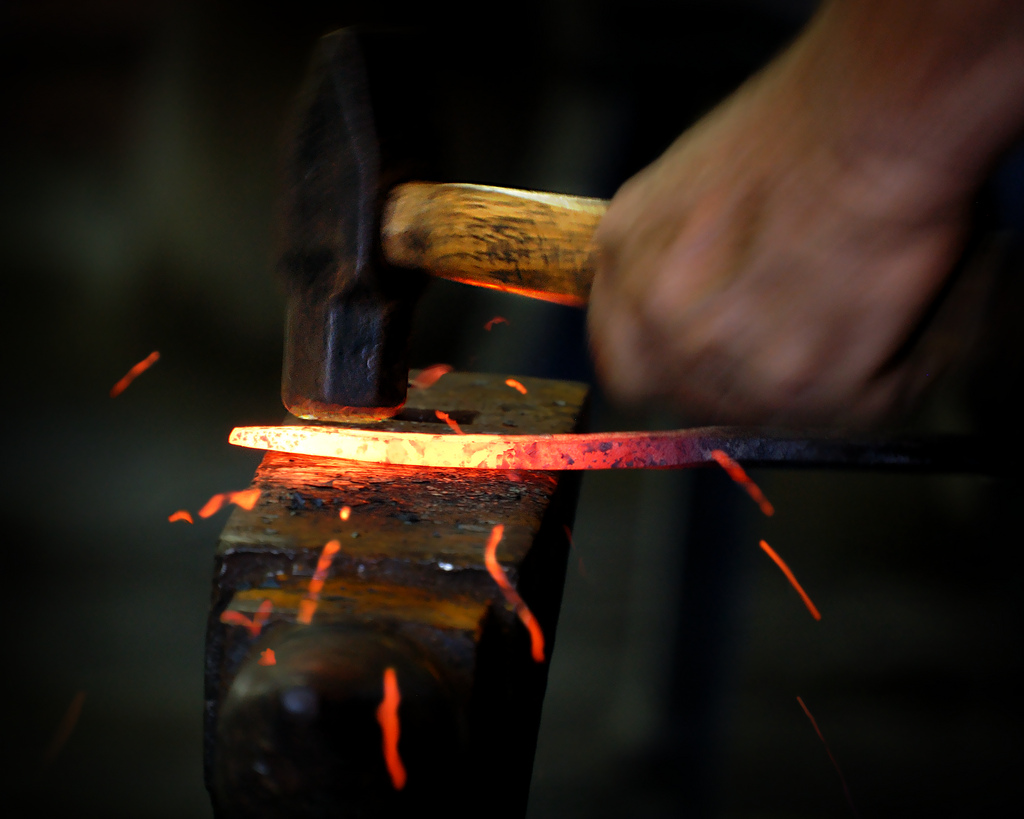
\includegraphics{res/Kovanje_zeljeza_l.jpg}
\caption[Kovanje željeza]{Kovanje željeza}
\label{figure:kovanje}
\end{figure}

\section{Algoritam}
Uvedimo nekoliko definicija:
\begin{itemize}
\item $S$ - trenutno stanje.

\item $S'$ - stanje koje je susjedno trenutnom.

\item $E(s)$ - funkcija koja računa energiju nekog stanja. Želimo pronaći
stanje s najmanjom (ili najvećom) energijom. 

\item $S_{n}$ - najbolje pronađeno stanje, tj. stanje u kojem je 
energija najmanja.

\item $e$ - energija trenutnog stanja, tj. $E(S)$.

\item $t$ - vrijeme proteklo od početka pokusa. 

\item $T$ - trenutna temperatura. Definiramo je kao $T_0 T_1^{t}$, gdje je
$T_0$ početna temperatura, a $T_1$ faktor koji govori koliko se temperatura
brzo smanjuje. 

\item $P(e, e', T)$ - vjerojatnost da prijeđemo u stanje koje ima energiju
$e'$ iz stanja koje ima energiju $e$ u trenutku $T$. 
\end{itemize}

Algoritam se sastoji od ponavljanja slijedećeg niza operacija
dok nismo dobili stanje koje ima traženu energiju ili dok vrijeme nije isteklo.

\begin{enumerate}
\item
Odaberi stanje $S'$ koje je susjedno stanju $S$. 

\item
Izračnaj energiju novog stanja $e' = E(S')$. 

\item 
Provjeri ima li novo stanje veću energiju od najboljeg do sada pronađenog stanja.
Ako ima, onda je $S_n = S'$.

\item
Izračunaj vjerojatnost napredovanja u stanje $S'$: $p = P(e, e', T)$. 

\item
Odaberi nasumičan broj iz intervala $[0, 1]$ i ako je manji od $p$, 
pomakni trenutno stanje u $S'$. 

\item 
Povećaj vrijeme $t$. 

\end{enumerate}

\subsection{Odabir susjeda}
U našem slučaju, odabir susjeda radimo tako uzmemo koordinate atoma te
im translatiramo sve tri koordinati, a cijeli niz potom rotiramo oko sve tri
osi. Time smo osigurali da možemo konstruirati bilo koji drugi izomorfan niz u
prostoru.

Da bismo bili sigurni da ne radimo prevelike skokove, svaka translacija
ili rotacija događa se u određenom intervalu, to jest,
nećemo raditi translacije koje za više od $x$ niti rotacije za više od
$\alpha$ stupnjeva.

\begin{figure}
\centering
\definecolor{qqqqff}{rgb}{0,0,1}
\begin{tikzpicture}[line cap=round,line join=round,>=triangle 45,x=1.0cm,y=1.0cm]
\clip(0.71,-1.14) rectangle (6.10,2.76);
\draw (1,1)-- (4,2)-- (6,0);
\draw (0.81,1.16)-- (3.59,2.66)-- (5.91,1.04);
\draw (1.16,0.81)-- (4.29,1.28)-- (5.91,-1.04);
\begin{scriptsize}
\fill [color=qqqqff] (1,1) circle (1.5pt);
\draw[color=qqqqff] (1.04,1.08) node {$A$};
\fill [color=qqqqff] (4,2) circle (1.5pt);
\draw[color=qqqqff] (4.04,2.08) node {$B$};
\fill [color=qqqqff] (6,0) circle (1.5pt);
\draw[color=qqqqff] (6.04,0.07) node {$C$};
\end{scriptsize}
\end{tikzpicture}
\caption[Rotacija nizova]{Slika prikazuje
maksimalu i minimalnu rotaciju nekog niza. Rotacija se radi oko
izvorišta. Iako radimo u 3D prosturu, za primjer je dana 2D
rotacija.}
\label{figure:susjed:rotacija}
\end{figure}

\begin{figure}
\centering
\definecolor{zzttqq}{rgb}{0.6,0.2,0}
\definecolor{qqqqff}{rgb}{0,0,1}
\begin{tikzpicture}[line cap=round,line join=round,>=triangle 45,x=1.0cm,y=1.0cm]
\clip(-1.10,-3.10) rectangle (7.10,5.10);
\fill[color=zzttqq,fill=zzttqq,fill opacity=0.1] (0,4) -- (0,-2) -- (2,-2) -- (5,-3) -- (7,-3) -- (7,3) -- (5,5) -- (3,5) -- cycle;
\draw (1,1)-- (4,2)-- (6,0);
\draw (0,-2)-- (3,-1)-- (5,-3);
\draw (2,4)-- (5,5)-- (7,3);
\draw (0,4)-- (3,5)-- (5,3);
\draw (2,-2)-- (5,-1)-- (7,-3);
\draw [color=zzttqq] (0,4)-- (0,-2);
\draw [color=zzttqq] (0,-2)-- (2,-2);
\draw [color=zzttqq] (2,-2)-- (5,-3);
\draw [color=zzttqq] (5,-3)-- (7,-3);
\draw [color=zzttqq] (7,-3)-- (7,3);
\draw [color=zzttqq] (7,3)-- (5,5);
\draw [color=zzttqq] (5,5)-- (3,5);
\draw [color=zzttqq] (3,5)-- (0,4);
\begin{scriptsize}
\fill [color=qqqqff] (1,1) circle (1.5pt);
\draw[color=qqqqff] (1.08,1.15) node {$A$};
\fill [color=qqqqff] (4,2) circle (1.5pt);
\draw[color=qqqqff] (4.09,2.15) node {$B$};
\fill [color=qqqqff] (6,0) circle (1.5pt);
\draw[color=qqqqff] (6.08,0.16) node {$C$};
\end{scriptsize}
\end{tikzpicture}
\caption[Translacija nizova]{Slika prikazuje
maksimalu i minimalnu translaciju nekog niza. 
Iako radimo u 3D prosturu, za primjer je dana 2D
translacija.}
\label{figure:susjed:translacija}
\end{figure}

\subsection{Računanje energije}
Za račuanje energije, koristimo prethodno opisani Smith-Waterman algoritam. 
Jedan ulazni niz je onaj koji želimo dobiti transformacijama, dok je drugi
onaj za kojeg računamo energiju. 
Budući da nam rekonstrukcija nije potrebna jer nas zanima samo energija,
nju niti ne računamo. Time ćemo dobiti ubrzanje od nekoliko puta.


\subsection{Računanje vjerojatnosti prihvaćanja}
Rješavanje ovog problema srž je algoritma simuliranog kaljenja. 
Jasno je da želimo otići u stanje koje ima bolju energiju, pa
će nam ova funkcija kada je nova energija veća od trenutne, uvijek
vratiti $1$, što znači da ćemo sigurno otići u to stanje. 
Ono što razlikuje ovaj algoritam od klasičnog algoritma
\textit{penjanja na brdo} (engl. \textit{hill-climbing}) jest 
ponašanje u slučaju da je nova energija manja od trenutne. 

Simulirano kaljenje, kao što je već rečeno, ponekad ode i u lošija
stanja. Hoće li se to dogoditi, ovisi o implementaciji funkcije
$P$. Kako nam inspiracija dolazi iz obrade metala, vjerojatnost da
prihvatimo loše stanje veća je na početku nego pri kraju. Također,
ako je rješenje puno lošije, ne isplati nam ga se prihvatiti kao
trenutno. 

Razmotrimo način na koji možemo modelirati vrijeme. Pretpostavimo
da nam $q$ označava trenutnu vrijednost funkcije $P$. Također,
uvedimo ograničenje da $q$ mora biti iz intervala $[0, 1]$.
Želimo, dakle, da $P$ pada kako vrijeme odmiče. Najjednostavnije
što možemo napraviti jest da od $q$ oduzmemo $t$. Međutim,
kako $P$ mora biti u granicama $[0, 1]$ to nije dobro rješenje.
Alternativno, ako oduzmemo $t/t_max$, dobili smo rješenje koje
je potencijalno u intervalu $[-1, 1]$ i linearno pada
ako mijenjamo samo vrijeme. Pokazalo se, međutim, da u "prirodi"
nije baš tako. Vjerojatnost, naime, pada eksponencijalno. 

Slično razmišljanje vrijedi i za modeliranje razlike u energiji.
Što je razlika veća, to nam vjerojatnost prijelaza treba biti manja.

Obično se uzima slijedeća funkcija: 
$$
P(e, e', T) = 
\left\{ \begin{array}{ll}
	1 & \mbox{ako je } e' > e \\
	\frac{1}{1+\exp \frac{e'-e}{T}} & \mbox{inače}
\end{array} \right.
$$
%TODO povećaj font u ovoj jednadžbi.

Primjetite da se, umjesto vremena, u njoj govori o temperaturi,
koja eksponencijalno pada kako vrijeme odmiče. 

\autoref{figure:vjerojatnost} daje graf funkcije $P(\Delta e, T)$, gdje
je $\Delta e = e'-e$. Os
$x$ predstavlja $\Delta e$, os $y$ je $T$ (bitno je ponoviti da
vremenom ova vrijednost pada) te os $z$ prikazuje vrijednost $P$. 
Budući da 3D graf prikazujemo na 2D površini, pobojali smo ga
u gradijent s obzirom na njegovu vrijednost kako bismo ga lakše 
interpretirali. 

% preuzeto s https://www.google.hr/search?hl=en&biw=1857&bih=995&noj=1&sclient=psy-ab&q=1%2F%281%2Be%5E%28x%2Fy%29%29&oq=1%2F%281%2Be%5E%28x%2Fy%29%29&aq=f&aqi=&aql=&gs_l=serp.3...274395.277370.0.277780.6.6.0.0.0.0.176.515.5j1.6.0...0.0.h3zpB1qjAkE
\begin{figure}
\centering
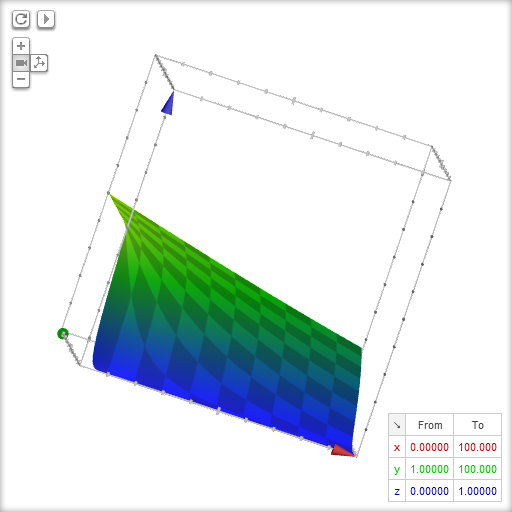
\includegraphics[scale=0.8]{res/P_graf_de(0_100)_t(1,100).PNG}
\caption[Graf funkcije $P$]{Graf funkcije vjerojatnosti prihvaćanja $P$.}
\label{figure:vjerojatnost}
\end{figure}

\section{Modifikacije}

Ovaj algoritam smo nešto prilagodili našoj upotrebi, kako bismo dobili
prihvatljivo rješenje što je moguće prije. Budući da je cijeli
algoritam baziran na heuristici, a izmjene koje smo napravili
ne utječu na točnost, smijemo ih koristiti jer jedina stvar
na što utječu su brzina algoritma. 

\subsection{Više susjeda}
Klasičan algoritam, kako je to gore objašnjeno, koristi samo jedan susjed u svakom
koraku. Mi ćemo u našem rješenju koristiti više ($k$) njih. Od tako dobivenih,
uzimamo onaj koji je najbolji i uspoređujemo ga, kako je gore opisano,
s trenutnim stanjem. 

\begin{figure}
\centering
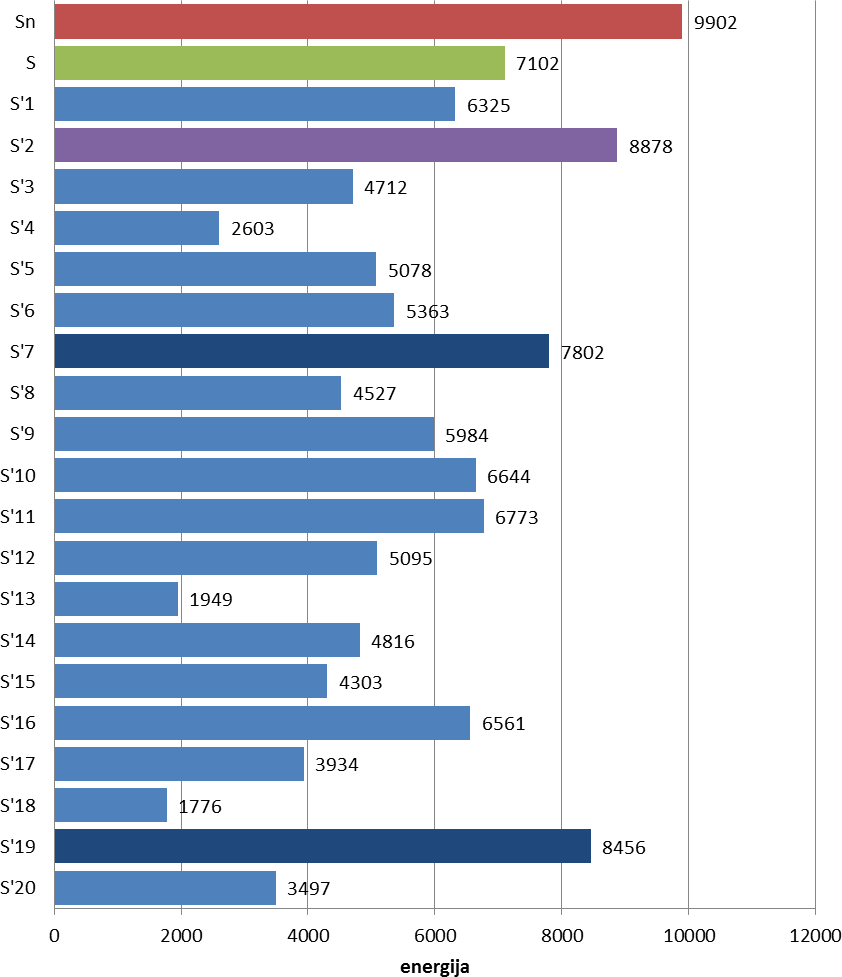
\includegraphics[scale=0.5]{res/energije_susjeda.png}
\caption[Korištenje više susjeda u algoritmu simuliranog kaljenja]{
Prikazan je slučaj kada imamo 20 susjeda. Energije svih susjeda koji
imaju energiju veću od trenutnog niza su označene tamno-plavom bojom,
a jedino je energija najvećeg susjeda, u koju ćemo premjestiti trenutno
stanje, pobojana u ljubičasto.}
\label{figure:susjedi}
\end{figure}

S obzirom da nam je svaki korak ocjenjivanja relativno skup, time se možemo
osigurati rijetko odlazimo u slabija stanja. Međutim, takav pohlepan
način odabira može nas dovesti u stanje lokalnog minimuma, iz kojeg se nećemo
izvući. Da bismo pokušali otkloniti taj problem, u 10\% genirirat ćemo samo jednog
susjeda u kojeg ćemo se, ako zadovljava uvjete, proširiti. 

Također, pokazat će se u nastavku, ovime možemo nešto uštedjeti i na korištenju
memorije i time povećati efikasnost koju dobijemo kada koristimo grafički
procesor za računanje traženih podataka. 

\subsection{Ponovo pokretanje}

Jedna od metoda da se izvučemo iz potencijalnog lokalnog ekstrema jest da
ponovo pokrenemo algoritam iz neke prethodne točke. Često se to implementira
na način da se promijeni vrijeme (smanji se, tj. postavi se u prošlost).
Time se poveća vjerojatnost da izađemo iz nekog lokalnog ekstrema koristeći
neka lošija stanja. 

U slučaju da se najbolje rješenje nije promjenilo u zadnjih 15 koraka, 
vrijeme ćemo resetirati da bismo se pokušali pomaknuti iz mogućeg lokalnog
ekstrema. 

\section{Parametari}

S obzirom da naglasak ovog rada nije bio isključivo na ovom algoritmu, 
a i na vremenske rokove postavljene na pisanje rada, parametri koji su se
koristili u implementaciji nisu previše istraženi. 






\chapter{CUDA tehnologija}
\textit{Compute Unified Device Architecture} (engl.; računski objedinjena
arhitektura uređaja) ili skraćeno CUDA, tehnologija je
koja nam omogućuje da upregnemo moć grafičkih čipova na
problemima za koje se tipično koristio CPU (odnosno procesor).
Kopanija Nvidija razvila ju je za svoje grafičke kartice. 

CUDA se smatra najnaprednijim alatom za općenamjensku uporabu
grafičke jedinice (engl. GPGPU - \textit{\textbf{g}eneral
\textbf{p}urpose \textbf{g}raphics \textbf{p}rocessing \textbf{u}nit}).
%TODO jos o ovome


Prva verzija CUDA-inog SDK-a (engl. \textit{\textbf{s}oftware
\textbf{d}evelopment \textbf{k}it} - oprema za razvoj programske
podrške) izdana je 15. veljače 2007.
Ona je omogućila korištenje resursa grafičkih kartica jedino u
programskom jeziku C. Od tada do danas izdane su još dvije velike
iteracije i nekoliko manjih te danas možemo koristiti i podskup
jezika C++. Osim službenog SDK-a, za čitav niz programskih jezika,
poput Fortrana, Jave, Haskella, Perla, Pythona, Matlaba, napisane su
neslužbene poveznice. 

%% preuzeto s http://en.wikipedia.org/wiki/File:CUDA_processing_flow_(En).PNG
%% protok podataka 
\begin{figure}
\centering
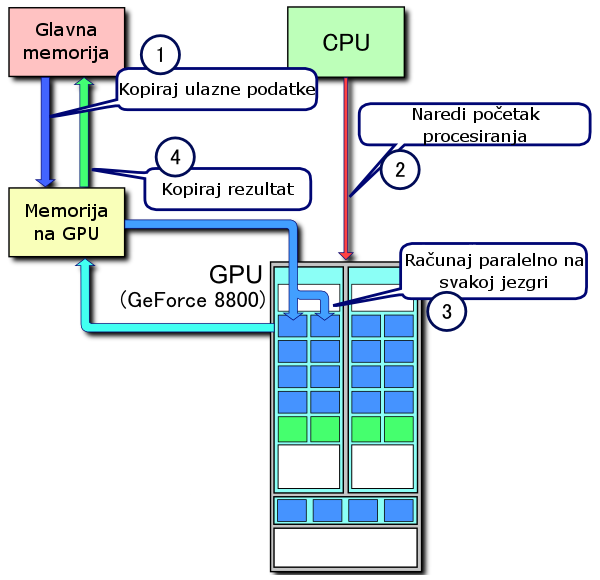
\includegraphics[scale=0.7]{res/CUDA_processing_flow_(hr).PNG}
\caption[Protok podataka na CUDA grafičkim karticama]{Protok podataka
na CUDA grafičkim karticama. Prvo iz glavne memorije računala (RAM-a)
kopiramo podatke u memoriju na GPU-u. Potom procesor naređuje
GPU-u da pokrene odgovarajući kernel na nekom broju jezgri. 
Kada one završe, rezultat se kopira nazad u glavnu memoriju.
CUDA SDK nas traži da ručno napravimo korake 1, 2 i 4, a on
se brine da se pravilno izvrši korak 3.}
\label{figure:cuda:dataflow}
\end{figure}


Pri radu na CUDA-i, moramo razumjeti slijedeće pojmove:
\begin{itemize}
\item
Domaćin (engl. \textit{host}) - računalo u kojem se nalazi grafička kartica.
Kada kažemo, npr. memorija domaćina mislimo na RAM. 

\item
Uređaj (engl. \textit{device}) - grafička kartica.

\item
(engl. \textit{grid}) - 
%TODO objasni

\item
Dretva (engl. \textit{thread}) - 

\item
(engl. \textit{warp}) -
%TODO objasni

%TODO dodaj jos nekoliko
\end{itemize}

Prednosti koje ova tehnologija (odnosno grafičke kartice koje su
sposobne koristiti ju) ima nad ostalim GPGPU tehnologijama
su slijedeće:
%TODO objasni sto je GPGPU

\begin{itemize}
\item
Nudi pristup bilo kojem dijelu memorije. 

\item
Dretve mogu koristiti brzu zajedničku dijelnu memoriju. 

\item
Podrška za račun s cijelobrojnim tipovima podataka, uključujući
i operacije s bitovima.
\end{itemize}

Nažalost, ništa u životu nije savršeno, pa tako nije niti CUDA.
Treba imati na umu da i ona ima i neka ograničenja:

\begin{itemize}
\item
Učestalo kopiranje memorije između uređaja i domaćina ima loš
utjecaj na brzinu izvođenja programa.

\item
U praksi se pokazalo da trebamo koristiti barem 32 dretve paralelno
da bismo dobili brži program nego onaj na CPU-u. Ukupan broj dretvi
koje koristimo trebao bi se brojati u tisućama. 

\item
Sklopovlje je dostupno isključivo od jednog proizvođača - Nvidije. 

\item
Zbog nezrelosti prevoditelja i optimizatora valjani C/C++ kôd
ne radi nužno i na CUDA-i. 

\item
Računanje s brojevima s posmačnim zarezom nije implementirano posve
po standardima, ali u većini slučajeva to ne igra nikakvu ulogu.
\end{itemize}







\chapter{Implementacija}

%TODO nacrtaj UML dijagram, ako ce trebati jos nekoliko stranica

\section{Implementacija simuliranog kaljenja}
Simulirano kaljenje temelji se na postupku koji je identičan
za sve tipove podataka. To nas navodi da implementaciju 
riješimo koristeći oblikovni obrazac okvirna metoda. 
Ideja tog oblikovnog obrasca jest da imamo jednu
metodu (funkciju) koja izvodi neki postupak pozivajući
generičke korake. Svaki korak može biti drugačije implementiran,
ovisno o postupku koji želimo. 

Izdvojimo apstraktne korake iz algoritma:
\begin{enumerate}
\item 
Odabir susjeda.

\item
Računanje energije stanja.

\item
Računanje vjerojatnosti prihvaćanja.
\end{enumerate}
Kako točno rješavamo svaki od tih koraka, napisalo smo u
prethodnom poglavlju. 

Implementacijski gledano, sva tri postupka su funkcije.
Prvi je funkcija koja prima jedan parametar, trenutno stanje
te vraća transformirano stanje koje dobijemo primjenjujući
translaciju i/ili rotaciju.
Drugi prima takvo transformirano stanje i računa njegovu
energiju. To radi tako da primjeni prethodno opisani
Smith-Waterman algoritam nad transforimarnim i ciljnem
nizom, ali ne radimo rekonstrukciju. 
Treći prima energiju početnog i krajenjeg niza te trenutnu
temperaturu te iz toga računa vjerojansto prihvaćanja
novog niza. 

Zahvaljujući genericima, tj. predlošcima, u C++ je lagano
ostaviriti ortogonalnost. Njihovom upotrebom, omogućavamo
da kôd algoritma napišemo samo jednom i da ga potom možemo
koristiti na više mjesta, za više tipova podataka,
što upravo i želimo. 

Takva implementacija omogućuje nam da ovaj dio programskog
rješenja testiramo i na nekom jednostavnijem problemu, što
uvelike olakšava razvoj programske potpore jer ne moramo
čekati za završetak cijelog sustava da bismo vidjeli radi li.
Osim toga, prilikom bubolova (engl. \textit{debugging}) nam
je lakše tražiti pogreške ako primjer možemo vizualizirati.
Nažalost, kako ovo nije problem u kojem je vizualizaciju
lagano napraviti, autor je koristio neke jednostavnije
probleme da bi ispravio pogreške u ovom dijelu koda. Primjeri
tih problema su traženje težišta poligona, %TODO jos bar dva primjera
Prilagodba algoritma za tu svrhu svela se na reimplantaciju
funkcija za računanje energije i odabir susjeda. 


\section{Implementacija Smith-Watermanovog algoritma}
Do sada smo razmatrali samo situaciju kada računamo jedno
po jedno polje matrice $R$. Pretpostavka je bila da su 
sva polja u prošlim retcima i trenutnom retku do trenutnog
stupca izračunata i da ih možemo koristiti u daljnjem
računu. 

Međutim, kada koristimo masivno paralalene procesore, 
želimo odjednonom računati više od jednog polja jer inače
ne uprežemo svu snagu koju nam oni nude.

Ideja na kojoj nam se temelji rješenje jest da primjetimo koja
su polja nezavisna, tj. koja možemo koristiti u računu ako
smo do sada već izračunali neki dio rješenja. Definirajmo
novu matricu $W$ u kojoj nam $W_{i,j}$ označava broj polja 
matrice $R$ koje moramo izračunati prije nego izračunamo
polje $R_{i,j}$. Na početku će vrijediti slijedeće:
$$
W_{i,j} = \left\{ \begin{array}{ll}
	0 & \mbox{ako je } i=0 \mbox{ i } j=0 \\
	3 & \mbox{ako je } i>0 \mbox{ i } j>0 \\
	1 & \mbox{inače}
\end{array} \right.
$$

\begin{table}
\centering
\begin{tabularx}{100pt}{|R|R|R|R|R|}
 \hline
 \cellcolor[rgb]{0.784314,0.784314,0.784314} 0 & 1 & 1 & 1 & 1 \\ \hline
 1 & 3 & 3 & 3 & 3 \\ \hline
 1 & 3 & 3 & 3 & 3 \\ \hline
 1 & 3 & 3 & 3 & 3 \\ \hline
 1 & 3 & 3 & 3 & 3 \\ \hline
\end{tabularx}
$\Rightarrow$
\begin{tabularx}{100pt}{|R|R|R|R|R|}
 \hline
 \cellcolor[rgb]{0.392157,0.392157,0.392157} 0 & \cellcolor[rgb]{0.784314,0.784314,0.784314} 0 & 1 & 1 & 1 \\ \hline
 \cellcolor[rgb]{0.784314,0.784314,0.784314} 0 & 2 & 3 & 3 & 3 \\ \hline
 1 & 3 & 3 & 3 & 3 \\ \hline
 1 & 3 & 3 & 3 & 3 \\ \hline
 1 & 3 & 3 & 3 & 3 \\ \hline
\end{tabularx}
$\Rightarrow$
\begin{tabularx}{100pt}{|R|R|R|R|R|}
 \hline
 \cellcolor[rgb]{0.392157,0.392157,0.392157} 0 & \cellcolor[rgb]{0.392157,0.392157,0.392157} 0 & \cellcolor[rgb]{0.784314,0.784314,0.784314} 0 & 1 & 1 \\ \hline
 \cellcolor[rgb]{0.392157,0.392157,0.392157} 0 & \cellcolor[rgb]{0.784314,0.784314,0.784314} 0 & 2 & 3 & 3 \\ \hline
 \cellcolor[rgb]{0.784314,0.784314,0.784314} 0 & 2 & 3 & 3 & 3 \\ \hline
 1 & 3 & 3 & 3 & 3 \\ \hline
 1 & 3 & 3 & 3 & 3 \\ \hline
\end{tabularx}
\caption[Matrica $W$]{Matrica $W$ na polju $W_{i,j}$ prikazuje broj polja koja
trebamo izračunati prije nego izračunamo polje $H_{i,j}$. Tamno-sivom bojom
prikazana su izračunata polja, a svijetlo-sivom ona koja možemo izračunati. }
\label{table:impl:sw:W}
\end{table}

Jasno je da možemo izračunati vrijednosti samo onih polja
za koje je $W_{i,j}=0$. Na početku je takvo samo jedno polje:
$W_{0,0}$. Međitim, kada njega izračunamo, smanjit ćemo
vrijednosti tri polja u matrici $W$: $W_{1,0}$, $W_{0,1}$ i
$W_{1,1}$. To će uzrokovati da $W_{1,0}$ i $W_{0,1}$ postanu
jednaki $0$, što znači da sada smijemo i njih izračanati.
Kada to učinimo, i osvježimo vrijednosti u matrici $W$, 
vidjet ćemo da smo dobili tri nove nule, na pozicijama
$W_{2,0}$, $W_{0,2}$ i $W_{1,1}$. Pravilnost se već
lagano počinje nazirati. Naime, sve elemente koji 
se nalaze na istoj sporednoj dijagonali moći ćemo 
izračunati u istom koraku. Stoga ćemo paralelizaciju
temeljiti upravo na tome da u pojedinom koraku
računamo sve elemente na sporednoj dijagonali. 

\begin{table}
\centering
\begin{tabularx}{240pt}{|R|R|R|R|R|R|R|R|R|R|R|R|}
 \hline
  &  &  &  &  &  &  &  &  & \cellcolor[rgb]{0.784314,0.784314,0.784314}  &  &  \\ \hline
  &  &  &  &  &  &  &  & \cellcolor[rgb]{0.784314,0.784314,0.784314}  &  &  &  \\ \hline
  &  &  &  &  &  &  & \cellcolor[rgb]{0.784314,0.784314,0.784314}  &  &  &  &  \\ \hline
  &  &  &  &  &  & \cellcolor[rgb]{0.784314,0.784314,0.784314}  &  &  &  &  &  \\ \hline
  &  &  &  &  & \cellcolor[rgb]{0.784314,0.784314,0.784314}  &  &  &  &  &  &  \\ \hline
  &  &  &  & \cellcolor[rgb]{0.784314,0.784314,0.784314}  &  &  &  &  &  &  &  \\ \hline
  &  &  & \cellcolor[rgb]{0.784314,0.784314,0.784314}  &  &  &  &  &  &  &  &  \\ \hline
  &  & \cellcolor[rgb]{0.784314,0.784314,0.784314}  &  &  &  &  &  &  &  &  &  \\ \hline
  & \cellcolor[rgb]{0.784314,0.784314,0.784314}  &  &  &  &  &  &  &  &  &  &  \\ \hline
 \cellcolor[rgb]{0.784314,0.784314,0.784314}  &  &  &  &  &  &  &  &  &  &  &  \\ \hline
  &  &  &  &  &  &  &  &  &  &  &  \\ \hline
\end{tabularx}
\caption[Prikaz sporedne dijagonale]{Prikazana je jedna od sporednih
dijagonala matrice. Sva polja na njoj možemo računati u istom trenutku.}
\label{table:impl:dijagonala}
\end{table}

%TODO prikaz vece matrice i dijagonala pofarbanih
% na njoj

Vremenska složenost takvog bi algoritma u optimalnom slučaju bila
bi $O(M+N)$. Nažalost, realan je slučaj daleko od optimalnog. 
Problem nam stvara to što nemamo dovoljno procesora da bismo
mogli pokrenuti računanja nad svim elmentima dijagonale, ako je
ona prevelika. Na sreću, CUDA nam ne stvara prevelike probleme
ako koristimo stvorimo više blokova (do najviše 65536) nego što
grafička kartica fizički može izračunati. S obzirom da dužina
nizova vjerojatno neće biti puno veća od 15000 elemenata, 
takvo ograničenje je sasvim prihvatljivo.

Isto tako, ako u memoriju grafičke kartice ne stanu
oba niza (što će se dogoditi, nasreću, samo za iznimno
duge nizove koje nećemo promatrati), morat ćemo prilagoditi
algoritam. Jedna efikasna ideja
za rješavanje tog problema jest da podijelimo nizove na manje
dijelove koje možemo u potpunosti riješiti te da kombiniramo
tako dobivena rješenja. 
Međutim, to izlazi izvan teme ovog rada, pa nećemo
ovdje detaljno objasniti kako se to radi.

Također, moramo biti svjesni da će konstanta koja je sakrivena u O
notaciji biti puno veća nego kod obične implementicje na procesoru,
budući da moramo koristiti barijere za sinkronizaciju. Pozivanje
funkcija također troši vrijeme, a i pristup globalnoj memoriji
uređaja jest skuplji nego pristup radnoj memoriji računala. 

Što se memorijske složenosti tiče, i nju možemo ovdje ostvariti
kao $O(M+N)$. Dovoljno nam je da, umjesto posljednja dva reda,
pamtimo posljednje tri sporedne dijagonale. Rekonstrukcija, iako nije potrebna
rješava se Hirschbergovim algoritmom. 





\chapter{Rezultati}
- cca 1-2 starnice







\chapter{Zaključak}
Zaključak.
- cca 1-2 stranice

- CUDA kao tehnologija jos je u zacecima, ali napreduje enormno brzo

- mnogo stavri je neistarzeno

- spomeni thrust i povuci paralelu s STL-om







\bibliography{literatura}{}
\bibliographystyle{fer}
% cca 2 stranice

\begin{sazetak}
Sažetak na hrvatskom jeziku.

\kljucnerijeci{Ključne riječi, odvojene zarezima.}
\end{sazetak}

% TODO: Navedite naslov na engleskom jeziku.
\engtitle{Title}
\begin{abstract}
Abstract.

\keywords{Keywords.}
\end{abstract}

\end{document}
